\documentclass[conference]{IEEEtran}
\usepackage{cite}
\usepackage{amsmath,amssymb,mathtools}
\usepackage{graphicx}
\usepackage{booktabs}
\usepackage{tikz}
\usetikzlibrary{arrows.meta,positioning,calc}
\usepackage{url}
\newcommand{\repourl}{https://github.com/Sayam2122/ME319-Assignment-2-Predictive-Tracking}
\newcommand{\dg}{^\circ}
\graphicspath{{../results/figures/}}
\hyphenation{man-oeuvre}

\begin{document}
\title{Predictive Tracking and Elevation-Axis Control of a Manoeuvring Aerial Object from Noisy Radar Data}
\author{\IEEEauthorblockN{Sayam Midha (24B2240), Piyush Meena (24B2275), Monaal Kumar Arya (24B2156),\\
Asmit Anand (24B2263), Shivam Gawande (24B2194)}
\IEEEauthorblockA{ME319 Control Systems, Autumn 2026 -- Assignment 2, IIT Bombay\\
Code: \texttt{\repourl}}}
\maketitle

\begin{abstract}
This report describes a system that points an elevation platform at the place where a manoeuvring target will be $T_p=0.5$ s from now. The radar gives noisy range and elevation at 20~Hz and can drop out for 0.5~s. We model the geared DC drive, estimate the target with an extended Kalman filter (Singer acceleration model), extrapolate the estimate to $t+T_p$, and follow the resulting angle with a PI compensator (phase margin $71.5\dg$, gain margin 6.4~dB). In three test scenarios the 0.5~s look-ahead pointing error is $0.15\dg$ RMS for a manoeuvring target, and a 0.5~s radar loss does not change it. A firing rule fires a laser pulse only when the estimated miss distance is small. All three scenarios and 10 of 10 unseen random cases were intercepted, assuming a pulse is judged against the target position at $t+T_p$.
\end{abstract}

\section{Introduction}
A laser or gun cannot be aimed at where the target is now, because the target moves before the shot arrives. It has to be aimed at where the target will be. This needs three things: a filter that estimates velocity and acceleration from noisy range and angle data, a predictor that still works when radar samples are missing, and a servo that follows the predicted angle. This report covers these three parts for one elevation axis in a 2-D plane (assignment ME319-A2 \cite{assign}).

\textbf{Objectives.} Track a target with measurement noise $\sigma_r=1$ m and $\sigma_\theta=0.02\dg$ at 20 Hz, predict its elevation $T_p=0.5$ s ahead, drive the platform with a linear compensator, and stay stable and accurate through manoeuvres and a 0.5 s sensor loss.

\textbf{Scope and assumptions.} The platform is treated as an ideal rigid, balanced, geared DC drive with a perfect encoder. Laser engagement follows the assignment: a pulse is a 0$\to$1 edge of \texttt{fire\_cmd}, pulses are at least 1 s apart, and a pulse hits if the beam passes within $R_{eng}=2$ m of the target. The assignment does not say which target position a pulse is judged against. We assumed the position at $t_{fire}+T_p$, because the platform points at the predicted position; the other reading (position at $t_{fire}$) is also reported. Quantities the assignment does not give are marked as our own choices.

\textbf{Approach.} The EKF with a Singer model and open-loop propagation gives the prediction, and a PI compensator is placed from the plant's integrator-plus-resonance shape. Estimator and firing-gate constants were chosen on a tuning set of random cases that is separate from the test cases.

\section{System Architecture and Design}
Fig.~\ref{fig:arch} shows the geometry and the signal flow. The radar, co-located with the platform, returns $(r,\theta)$ every 50 ms. The EKF runs only when a new sample arrives. Between samples, and during a loss, the predictor propagates the last estimate with the same motion model, so the reference never stalls. The predicted position $(x_p,y_p)$ at $t+T_p$ is converted to $\theta_{ref}=\operatorname{sat}\big(\operatorname{atan2}(y_p,x_p)\big)$ limited to $[-10\dg,85\dg]$. The error $e=\theta_{ref}-\theta$ drives the compensator $G_c(s)$, whose output (saturated, with anti-windup) is the motor voltage.

\begin{figure*}[t]
\centering
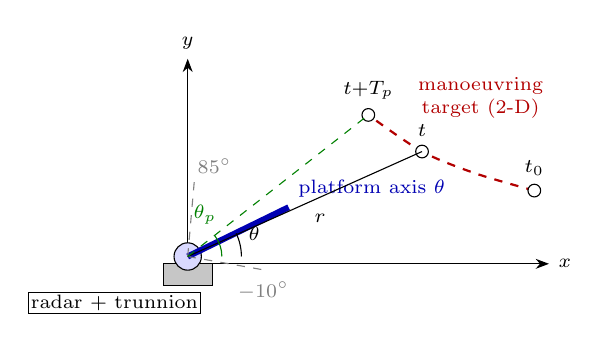
\begin{tikzpicture}[scale=0.62,>=Stealth,every node/.style={font=\scriptsize}]
\draw[->] (0,0)--(7.4,0) node[right]{$x$}; \draw[->] (0,0)--(0,4.2) node[above]{$y$};
\fill[gray!45] (-0.5,-0.45) rectangle (0.5,0); \draw (-0.5,-0.45) rectangle (0.5,0);
\draw[fill=blue!15] (0,0.15) circle (0.28);
\draw[line width=2.2pt,blue!70!black] (0,0.15)--({2.3*cos(26)},{0.15+2.3*sin(26)});
\node[blue!70!black,above right] at ({2.3*cos(26)},{0.15+2.3*sin(26)}) {platform axis $\theta$};
\draw[dashed,gray] (0,0.15)--({1.7*cos(-10)},{0.15+1.7*sin(-10)}); \draw[dashed,gray] (0,0.15)--({1.7*cos(85)},{0.15+1.7*sin(85)});
\node[gray] at (1.55,-0.55) {$-10\dg$}; \node[gray] at (0.55,2.0) {$85\dg$};
\node[draw,fill=white,inner sep=1pt] at (-1.5,-0.8) {radar + trunnion};
\draw[red!70!black,dashed,thick] plot[smooth] coordinates {(7.1,1.5)(5.9,1.85)(4.8,2.3)(3.7,3.05)};
\foreach \p/\n in {(7.1,1.5)/{$t_0$},(4.8,2.3)/{$t$},(3.7,3.05)/{$t{+}T_p$}} {\draw[fill=white] \p circle (0.13); \node[above=2pt] at \p {\n};}
\draw (0,0.15)--(4.8,2.3) node[midway,below right] {$r$};
\draw[green!50!black,dashed] (0,0.15)--(3.7,3.05);
\draw (1.1,0.15) arc (0:25.5:1.1) node[right,xshift=1pt] {$\theta$};
\draw[green!50!black] (0.7,0.15) arc (0:38:0.7); \node[green!50!black] at (0.35,1.0) {$\theta_p$};
\node[align=center,red!70!black] at (6.0,3.4) {manoeuvring\\target (2-D)};
\end{tikzpicture}\hfill
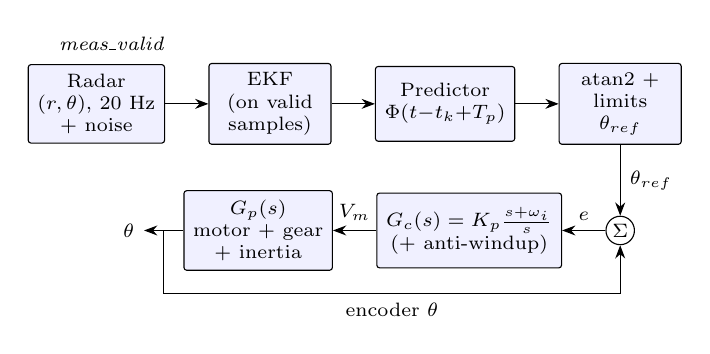
\begin{tikzpicture}[scale=1,>=Stealth,every node/.style={font=\scriptsize},blk/.style={draw,rounded corners=1pt,minimum height=0.95cm,minimum width=1.55cm,align=center,fill=blue!6},node distance=0.55cm]
\node[blk] (rad) {Radar\\$(r,\theta)$, 20 Hz\\+ noise};
\node[blk,right=of rad] (ekf) {EKF\\(on valid\\samples)};
\node[blk,right=of ekf] (pred) {Predictor\\$\Phi(t{-}t_k{+}T_p)$};
\node[blk,right=of pred] (ref) {atan2 +\\limits\\$\theta_{ref}$};
\node[circle,draw,inner sep=1pt,below=0.9cm of ref] (sum) {$\Sigma$};
\node[blk,left=of sum] (gc) {$G_c(s)=K_p\frac{s+\omega_i}{s}$\\(+ anti-windup)};
\node[blk,left=of gc] (gp) {$G_p(s)$\\motor + gear\\+ inertia};
\node[left=0.5cm of gp] (th) {$\theta$};
\draw[->] (rad)--(ekf); \draw[->] (ekf)--(pred); \draw[->] (pred)--(ref);
\draw[->] (ref)--(sum) node[midway,right] {$\theta_{ref}$};
\draw[->] (sum)--(gc) node[midway,above] {$e$};
\draw[->] (gc)--(gp) node[midway,above] {$V_m$};
\draw[->] (gp)--(th);
\draw[->] ($(gp.west)+(-0.25,0)$) |- ++(0,-0.8) -| node[pos=0.25,below] {encoder $\theta$} (sum.south) ;
\node[above=0.05cm of rad,xshift=0.2cm] {\textit{meas\_valid}};
\end{tikzpicture}
\caption{Left: elevation-plane geometry (target at $t_0$, $t$ and predicted $t{+}T_p$). Right: predictive-feedback block diagram.}
\label{fig:arch}
\end{figure*}

\subsection{Firing logic}
The firing rule sits inside \texttt{turret\_controller} and uses only what the controller knows. Let $\theta_p$ and $r_p$ be the predicted elevation and range at $t+T_p$, and $\sigma_{\theta_p}$ the EKF standard deviation of $\theta_p$. A pulse is issued only if (1) at least 1 s has passed since the last pulse, (2) $t\ge0.5$ s, (3) $\theta_p$ is inside the mechanical range, (4) the estimated miss $\hat m=r_p|\sin(\theta_p-\theta)|\le k_gR_{eng}$, and (5) $r_p\sigma_{\theta_p}\le k_\sigma R_{eng}$, with $k_g=0.50$ and $k_\sigma=1.50$. Test (4) uses the pointing error the loop actually has. Test (5) stops firing when the estimate is poor, for example just after start-up or during a radar loss. Firing only when the gate is open is better than firing every second, because each pulse costs a 1 s recharge. The constants $k_g,k_\sigma$ were picked on the tuning set and then fixed.

\section{Mathematical Modelling}
\subsection{Elevation drive}
Let $\omega=\dot\theta$, motor speed $\omega_m=N\omega$ ($N=100$), armature current $i$ and voltage $V_m$. Kirchhoff's voltage law, the motor torque law, ideal gearing ($T_{load}=NT_m$) and Newton's law for the platform give
\begin{align}
L_m\dot i + R_m i + K_eN\omega &= V_m, \qquad T_m=K_t i,\label{eq:elec}\\
J_{turret}\dot\omega + b\omega &= N T_m - N^2 J_m\dot\omega .\label{eq:mech}
\end{align}
The rotor inertia reflects to the platform as $N^2J_m$, so
\begin{equation}
J_{eq}\dot\omega + b\omega = NK_t\, i,\quad J_{eq}=J_{turret}+N^2J_m=3200~\mathrm{kg\,m^2}.\label{eq:jeq}
\end{equation}
Laplace transformation with zero initial conditions gives $(L_ms+R_m)I=V-K_eNs\Theta$ and $(J_{eq}s+b)s\Theta=NK_tI$, hence
\begin{equation}
\begin{split}G_p(s)&=\frac{\Theta}{V}\\&=\frac{NK_t}{s\big[L_mJ_{eq}s^2+(R_mJ_{eq}+L_mb)s+R_mb+N^2K_tK_e\big]}\end{split}\label{eq:gp}
\end{equation}
With the given data $G_p=1000/(320s^3+3350s^2+1.0015{\times}10^6s)$, i.e.\ an integrator times a resonant pair at $\omega_n=55.9$ rad/s, $\zeta=0.094$ (poles $-5.23\pm j55.7$). Below $\omega_n$, $G_p\approx K_v/s$ with $K_v=NK_t/(R_mb+N^2K_tK_e)=9.985e-04$ rad/s/V; the back-emf term $N^2K_tK_e=10^6$ dominates the 1500 N\,m\,s/rad damping. In state-space form with $\mathbf x=[\theta\ \omega\ i]^T$:
\begin{equation}
\dot{\mathbf x}=\begin{bmatrix}0&1&0\\0&-\tfrac{b}{J_{eq}}&\tfrac{NK_t}{J_{eq}}\\0&-\tfrac{K_eN}{L_m}&-\tfrac{R_m}{L_m}\end{bmatrix}\mathbf x+\begin{bmatrix}0\\0\\\tfrac1{L_m}\end{bmatrix}V_m,\; y=\theta .
\end{equation}
\textit{Assumptions:} rigid, backlash-free gearing; balanced platform (no gravity torque, so the model is the same at every operating angle and the small-perturbation model equals the full model); linear viscous damping; ideal encoder; end-stops enforced separately. \textit{Dimensions:} every term of \eqref{eq:elec} is in volts and every term of \eqref{eq:mech} in N\,m ($[K_t]=[K_e]=\mathrm{N\,m/A}=\mathrm{V\,s/rad}$); this and an energy balance of the simulated plant (residual $10^{-6}$) are automated checks in the repository.

\subsection{Target and sensor}
The target position is $(x,y)$, range $r=\sqrt{x^2+y^2}$, elevation $\theta_t=\operatorname{atan2}(y,x)$. Measurements are $z=[r;\theta_t]+v$, $v\sim\mathcal N(0,R)$, $R=\mathrm{diag}(\sigma_r^2,\sigma_\theta^2)$. Scenarios use bounded smooth accelerations $a(t)=A\sin(\omega_m(t-t_m)+\phi)\,s(t)$, with $s$ a smoothstep ramp, enforced to satisfy $800\le r\le2000$ m, $|v|\le150$ m/s, $|a|\le20$ m/s$^2$.

\section{State Estimation and Prediction}
\textbf{Model.} Each Cartesian axis follows a Singer model, $\dot{\mathbf s}=A_c\mathbf s+G w$, $\mathbf s=[p\ v\ a]^T$, $A_c=\begin{bsmallmatrix}0&1&0\\0&0&1\\0&0&-\alpha\end{bsmallmatrix}$, $G=[0\ 0\ 1]^T$, $E[w(t)w(\tau)]=q\delta(t-\tau)$; the full state is $\mathbf X=[x\ v_x\ a_x\ y\ v_y\ a_y]^T$. Acceleration is thus a zero-mean first-order Gauss--Markov process (stationary std $\sqrt{q/2\alpha}=7.1$ m/s$^2$, correlation time $1/\alpha$), appropriate for a manoeuvring target whose acceleration is bounded and does not persist \cite{singer,li}. The transition matrix over $\Delta$ is
\begin{equation}
\Phi_1(\Delta)=\begin{bmatrix}1&\Delta&\tfrac{\alpha\Delta-1+e^{-\alpha\Delta}}{\alpha^2}\\0&1&\tfrac{1-e^{-\alpha\Delta}}{\alpha}\\0&0&e^{-\alpha\Delta}\end{bmatrix},\;F=\mathrm{blkdiag}(\Phi_1,\Phi_1),
\end{equation}
and $Q(\Delta)=\int_0^\Delta \Phi\, GqG^T\Phi^T d\tau$ per axis (computed with Van Loan's method \cite{vanloan}).

\textbf{EKF.} Time update: $\hat X^-=F(\Delta)\hat X$, $P^-=FPF^T+Q(\Delta)$, with $\Delta=t-t_{k}$ the \emph{actual} elapsed time (so a missed sample inflates $P$ correctly). Measurement update with $h(X)=[\sqrt{x^2+y^2};\operatorname{atan2}(y,x)]$ and Jacobian $H=\begin{bsmallmatrix}x/\rho&0&0&y/\rho&0&0\\-y/\rho^2&0&0&x/\rho^2&0&0\end{bsmallmatrix}$, $\rho^2=x^2+y^2$:
\begin{align}
K&=P^-H^T(HP^-H^T+R)^{-1},\quad \hat X=\hat X^-+K\nu,\\
P&=(I-KH)P^-(I-KH)^T+KRK^T,
\end{align}
where $\nu=z-h(\hat X^-)$ with the angle residual wrapped (Joseph form keeps $P$ positive semidefinite). \textbf{Initialisation:} the first sample gives position by polar-to-Cartesian conversion with covariance $JRJ^T$; velocity and acceleration start at zero with prior std equal to the admissible bound over $\sqrt3$ (uniform prior on $[-v_{max},v_{max}]$, $[-a_{max},a_{max}]$), i.e.\ 86.6 m/s and 11.5 m/s$^2$.

\textbf{Prediction.} With the latest update at $t_k$, $\hat X(t+T_p)=F(t-t_k+T_p)\hat X_k$; this needs no new data, so it continues unchanged through a loss. The reference is $\theta_{ref}=\operatorname{sat}(\operatorname{atan2}(\hat y_p,\hat x_p))$. Its uncertainty is obtained from $P$ propagated over the same interval and the gradient of $\operatorname{atan2}$.

\textbf{Parameter selection.} $q$ and $\alpha$ were chosen on 16 random bounded manoeuvres (half with a loss), disjoint from scenarios A--C and from the test cases of Sec.~VI, by minimising the RMS 0.5~s-ahead elevation error over a $5\times5$ grid. The error surface has a flat ridge; its grid minimum 0.0612$\dg$ is at $(q,\alpha)=(200,2)$, the values frozen in the code (the neighbouring $(600,4)$ is within 1\%). A constant-acceleration model ($\alpha=0$, same $q$) gives 0.0761$\dg$, i.e.\ the decay term helps. Consistency: the mean normalised innovation squared is 1.64 (A) and 1.86 (B) against the expected value 2 for two measurements.

\section{Controller Design and Stability Analysis}
\textbf{Structure.} Because $G_p\approx K_v/s$ below $\omega_n$, a PI compensator $G_c(s)=K_p(s+\omega_i)/s$ gives a type-2 loop: zero steady-state error for a ramp reference (target at constant angular rate) and error $e_{ss}=\ddot\theta_{ref}/K_a$ with $K_a=\lim s^2L=K_pK_v\omega_i=8.33$ s$^{-2}$ for constant angular acceleration. With $\omega_c\ll\omega_n$, $|L(j\omega_c)|\approx K_pK_v/\omega_c=1$ gives $K_p=\omega_c/K_v$, and the phase margin is about $\arctan(\omega_c/\omega_i)$ minus a small resonance lag.

\textbf{Choice of $\omega_c$.} The resonance bounds the bandwidth: $|L(j\omega_n)|\approx(\omega_c/\omega_n)/(2\zeta)$ must stay below 1 for gain stabilisation. For $\omega_c=5.0$ rad/s this is $\approx0.48$ ($\approx6$ dB). Larger $\omega_c$ erodes the gain margin (e.g.\ 2.3 dB at 8 rad/s in the design sweep) while the reference spectrum (manoeuvre periods $\ge1.5$ s) lies at or below $\sim4$ rad/s. A notch at $\omega_n$ would permit more bandwidth but depends on an exactly known resonance, so we preferred the simpler gain-stabilised design. With $\omega_i=\omega_c/3$:
\begin{equation}
G_c(s)=5008\,\frac{s+1.67}{s},\; L(s)=G_c(s)G_p(s).
\end{equation}

\textbf{Closed loop and stability.} $T=L/(1+L)$ and the characteristic equation is
\begin{equation}
\begin{split}&320s^4+3350s^3+1.0015{\times}10^6s^2\\&\;+1000K_ps+1000K_p\omega_i=0.\end{split}
\end{equation}
The Routh array has a positive first column for the chosen $K_p$; its last entry gives the exact gain limit $K_{p,max}=a_3(a_2-a_3\omega_i)/(a_4\,NK_t)=10426$ V/rad, i.e.\ $\mathrm{GM}=6.37$ dB, which matches the numerical margin $6.4$ dB. Phase margin is $71.5\dg$ at $\omega_{gc}=5.29$ rad/s; the closed-loop poles are $-2.71\pm j55.6$ (resonant pair, damping reduced from $0.094$ to $0.049$) and $-2.52\pm j1.44$ (dominant, $\zeta\approx0.87$). The step response has 17.6\% overshoot (from the PI zero), 0.25 s rise time and 1.79 s 2\% settling time (Fig.~\ref{fig:ctrl}); $|T(j1)|=1.10$ and the $-3$ dB bandwidth is 6.8 rad/s. $M_s=5.72$ dB.

\textbf{Noise, prediction error, loss, limits.} The transfer from reference to voltage is $G_cS\to K_p=5008$ V/rad at high frequency, so reference jitter of $10^{-3}$ rad costs about 5 V, small against the $\ge$50 V used for tracking; the EKF smoothing (raw position error 1.05 m $\to$ 0.56 m) is therefore the main noise defence, and no derivative action is used. Prediction error enters additively on $\theta_{ref}$ and is passed by $T(s)$, so the look-ahead error is approximately the sum of the prediction error and the tracking error. During a loss the reference is generated open-loop; it is smooth, so the loop sees no discontinuity, and the first valid sample after recovery re-corrects it. $\theta_{ref}$ is clipped to the mechanical range, the voltage is limited ($V_{sat}=1500$ V, an assumption since none is given) with conditional-integration anti-windup, and hard end-stops are simulated.

\begin{figure*}[t]
\centering
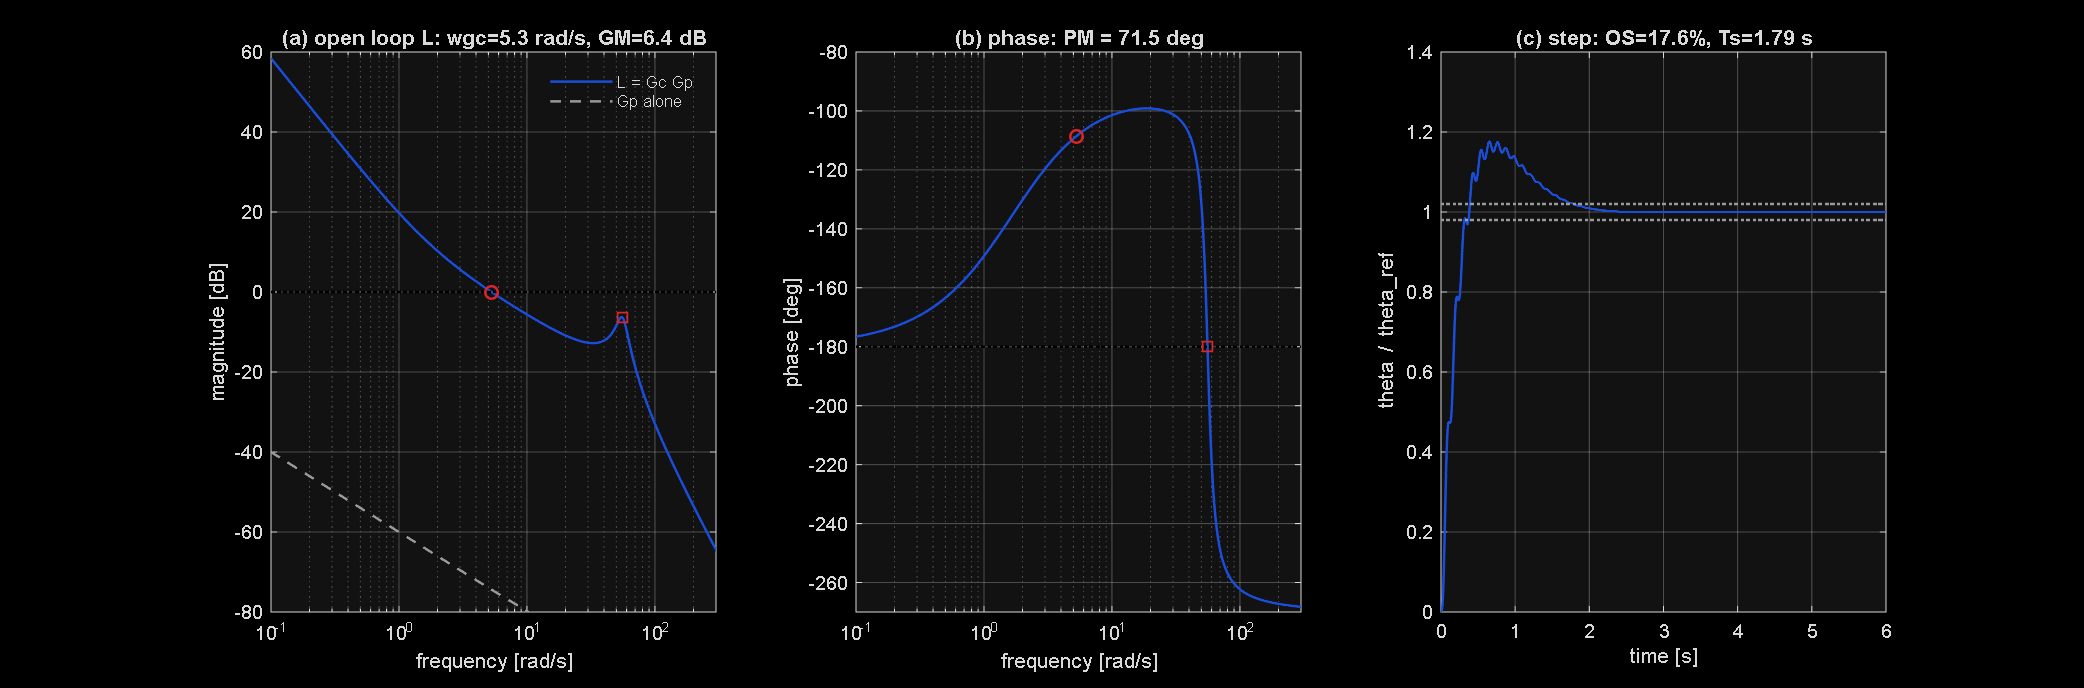
\includegraphics[width=0.66\textwidth]{fig_controller.png}\hfill
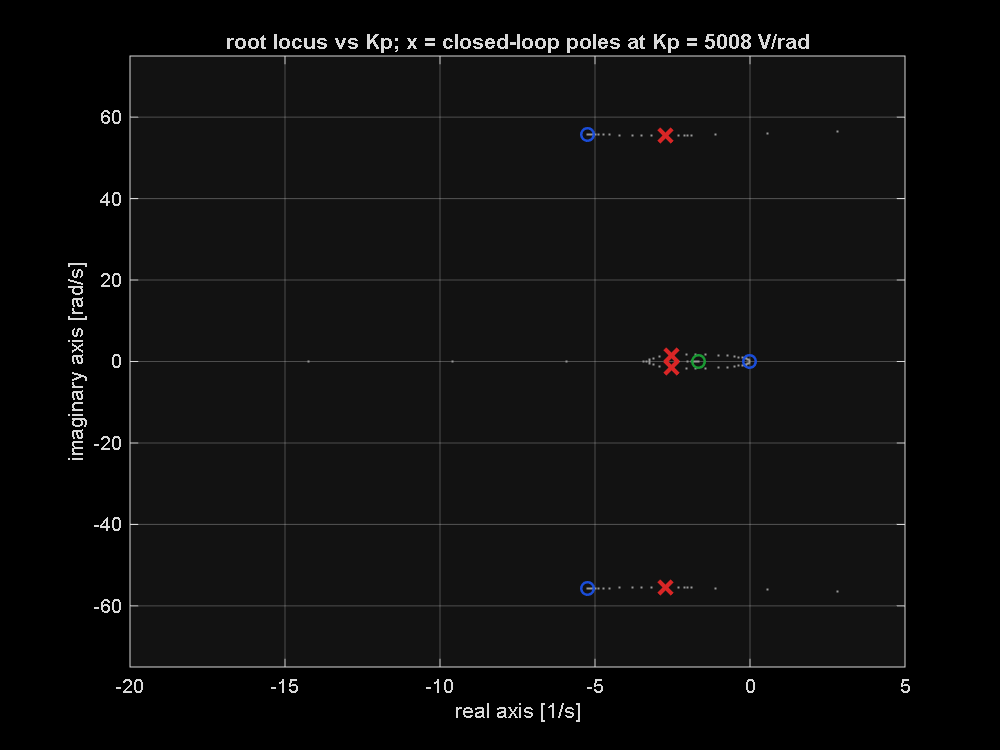
\includegraphics[width=0.31\textwidth]{fig_rootlocus.png}
\caption{Loop analysis: (a,b) Bode magnitude/phase of $L=G_cG_p$ with gain-crossover (o) and phase-crossover (square); (c) unit step response of $T$; right: root locus versus $K_p$ (red x: chosen $K_p$).}
\label{fig:ctrl}
\end{figure*}

\section{Simulation and Results}
\textbf{Set-up.} Octave 8.4 (MATLAB-compatible), 1 kHz RK4 integration of the actual \texttt{turret\_plant}, ZOH voltage, 20 Hz radar, 10 s. Platform starts aligned with the target. Scenario A: constant velocity $(-90,0)$ m/s from $(1800,500)$ m. B: same, plus smooth accelerations ($12$ and $14$ m/s$^2$ amplitude, periods 6 and 4.5 s) from $t=1$ s. C: B with the radar lost for $[1.0,1.5)$ s. Noise is generated by a portable Park--Miller generator \cite{parkmiller} with a fixed seed. Metrics use $t\ge1$ s unless stated (the first second is estimator acquisition); full-interval values are in \texttt{results/data}.

\begin{table}[t]
\centering\caption{Performance, $t\ge 1$ s (generated by the code)}\label{tab:perf}
\scriptsize\resizebox{\columnwidth}{!}{\begin{tabular}{lccc}
\toprule
Metric ($t\ge 1$ s) & A & B & C \\
\midrule
EKF position error, RMS [m] & 0.56 & 0.68 & 0.98 \\
Raw radar position error, RMS [m] & 1.05 & 1.05 & 1.06 \\
EKF velocity error, RMS [m/s] & 1.69 & 3.07 & 3.40 \\
Prediction error $\theta_p-\theta(t{+}T_p)$, RMS [deg] & 0.038 & 0.101 & 0.101 \\
Prediction error, max [deg] & 0.126 & 0.256 & 0.256 \\
Tracking error $\theta_{ref}-\theta$, RMS [deg] & 0.041 & 0.070 & 0.071 \\
Tracking error, max [deg] & 0.142 & 0.205 & 0.205 \\
Look-ahead error $\theta(t{+}T_p)-\theta$, RMS [deg] & 0.035 & 0.150 & 0.149 \\
Look-ahead error, max [deg] & 0.125 & 0.297 & 0.297 \\
\midrule
Peak motor voltage [V] & 53 & 37 & 37 \\
Peak motor current [A] & 3.63 & 3.63 & 3.63 \\
\bottomrule
\end{tabular}}
\end{table}

\textbf{Estimation.} Fig.~\ref{fig:est} shows scenario B. The EKF reduces the position error from 1.05 m (raw) to 0.56 m (A) and 0.68 m (B); the velocity error is 1.69 m/s (A) and 3.07 m/s (B). The larger values in B are the manoeuvre lag. Velocity is recovered from position data alone.

\textbf{Prediction and loss.} Prediction error is 0.038$\dg$ RMS in A and 0.101$\dg$ in B (Fig.~\ref{fig:pred}). In C the maximum prediction error inside the loss window plus horizon ($1.0$--$2.0$ s) is 0.112$\dg$ (position 5.04 m), and the EKF's own predicted $1\sigma$ reaches 0.144$\dg$, so the covariance honestly reports the degradation; the estimate returns within $3\sigma_r$ at the first valid sample (recovery time 0.00 s). Whole-run metrics of C equal those of B to three digits because the loss starts when the manoeuvre acceleration has barely ramped up (0.150 vs.\ 0.149$\dg$). This is the \emph{mildest} admissible timing, so a sweep over the loss onset was run (below).

\textbf{Pointing.} The platform follows the reference with RMS error 0.070$\dg$ (B), and the look-ahead error $\theta(t{+}T_p)-\theta$ is 0.035$\dg$ (A), 0.150$\dg$ (B) and 0.149$\dg$ (C) RMS, maxima 0.125, 0.297 and 0.297$\dg$ (Fig.~\ref{fig:turret}). Peak voltage is 37 V and peak current 3.63 A (dominated by the start-up transient), far from $V_{sat}$.

\textbf{Engagement.} Table~\ref{tab:eng} and Fig.~\ref{fig:eng} show the pulses. The gate waits until the estimate has settled and the platform is close to the predicted target, so 9, 8 and 8 pulses are fired in A, B and C. The first hit is at 0.95 s in all three, with misses of 1.11, 0.80 and 0.80 m. The limit is geometric: 2 m is $0.115\dg$ at 1 km but only $0.057\dg$ at 2 km, while the look-ahead RMS error in B is $0.15\dg$. So at long range a hit happens only when the prediction error and the tracking error are both small at that moment.

\begin{table}[t]
\centering\caption{Laser engagement, scenarios A--C}\label{tab:eng}
\scriptsize\begin{tabular}{lccc}
\toprule
Engagement & A & B & C \\
\midrule
Pulses fired & 9 & 8 & 8 \\
Intercepted (miss $\le R_{eng}$) & yes & yes & yes \\
Interception time [s] & 0.95 & 0.95 & 0.95 \\
Miss at first hit [m] & 1.11 & 0.80 & 0.80 \\
\bottomrule
\end{tabular}
\end{table}
\begin{figure}[t]
\centering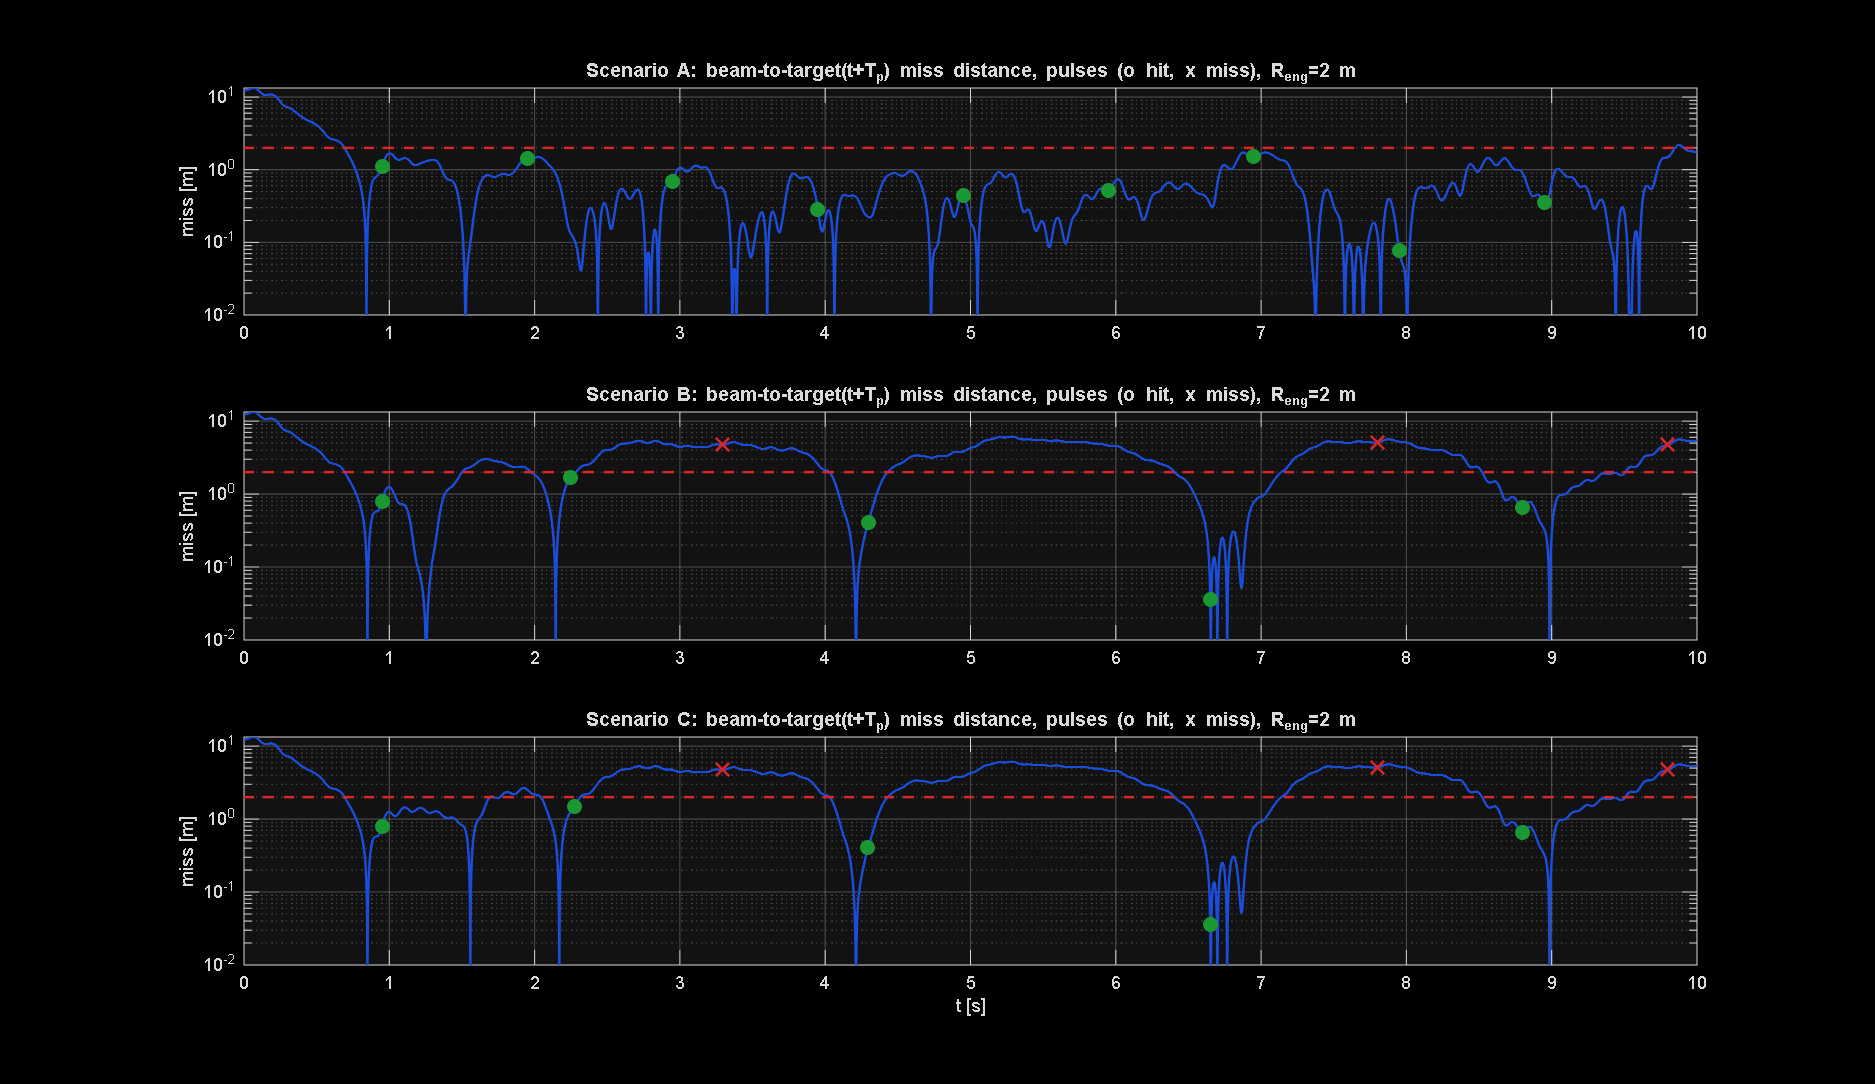
\includegraphics[width=\columnwidth]{fig_engagement.png}
\caption{Beam-to-target$(t{+}T_p)$ miss distance, pulses (o hit, x miss) and $R_{eng}$ (dashed).}\label{fig:eng}
\end{figure}

\textbf{Generalisation.} We ran the frozen design, with no retuning, on 10 random manoeuvres (half with a radar loss of up to 0.5 s starting after 1 s). The look-ahead RMS error averages $0.089\dg$ (worst $0.137\dg$), the maximum error averages $0.225\dg$ (worst $0.348\dg$), the worst prediction error is $0.324\dg$ and the worst voltage is 189 V, so the voltage limit was never reached (Fig.~\ref{fig:rob}a). All 10 cases were intercepted, with a mean interception time of 0.81 s (worst 1.80 s), a worst miss of 1.60 m at the hit, and 9.4 pulses per case, of which 82\% hit. Most first hits come early because the target has not started to manoeuvre yet ($t_{man}\ge1$ s), so the 82\% per-pulse figure says more about consistency. If a pulse were judged against the target at $t_{fire}$ instead, only 2 of 10 cases would be intercepted. Moving a 0.5 s loss across the scenario-B manoeuvre (Fig.~\ref{fig:rob}b), the worst prediction error in the window is $0.457\dg$ (onset 7.5 s) against $0.228\dg$ without a loss. A loss at peak acceleration roughly doubles the error but does not make the loop unstable.

\begin{figure*}[t]
\centering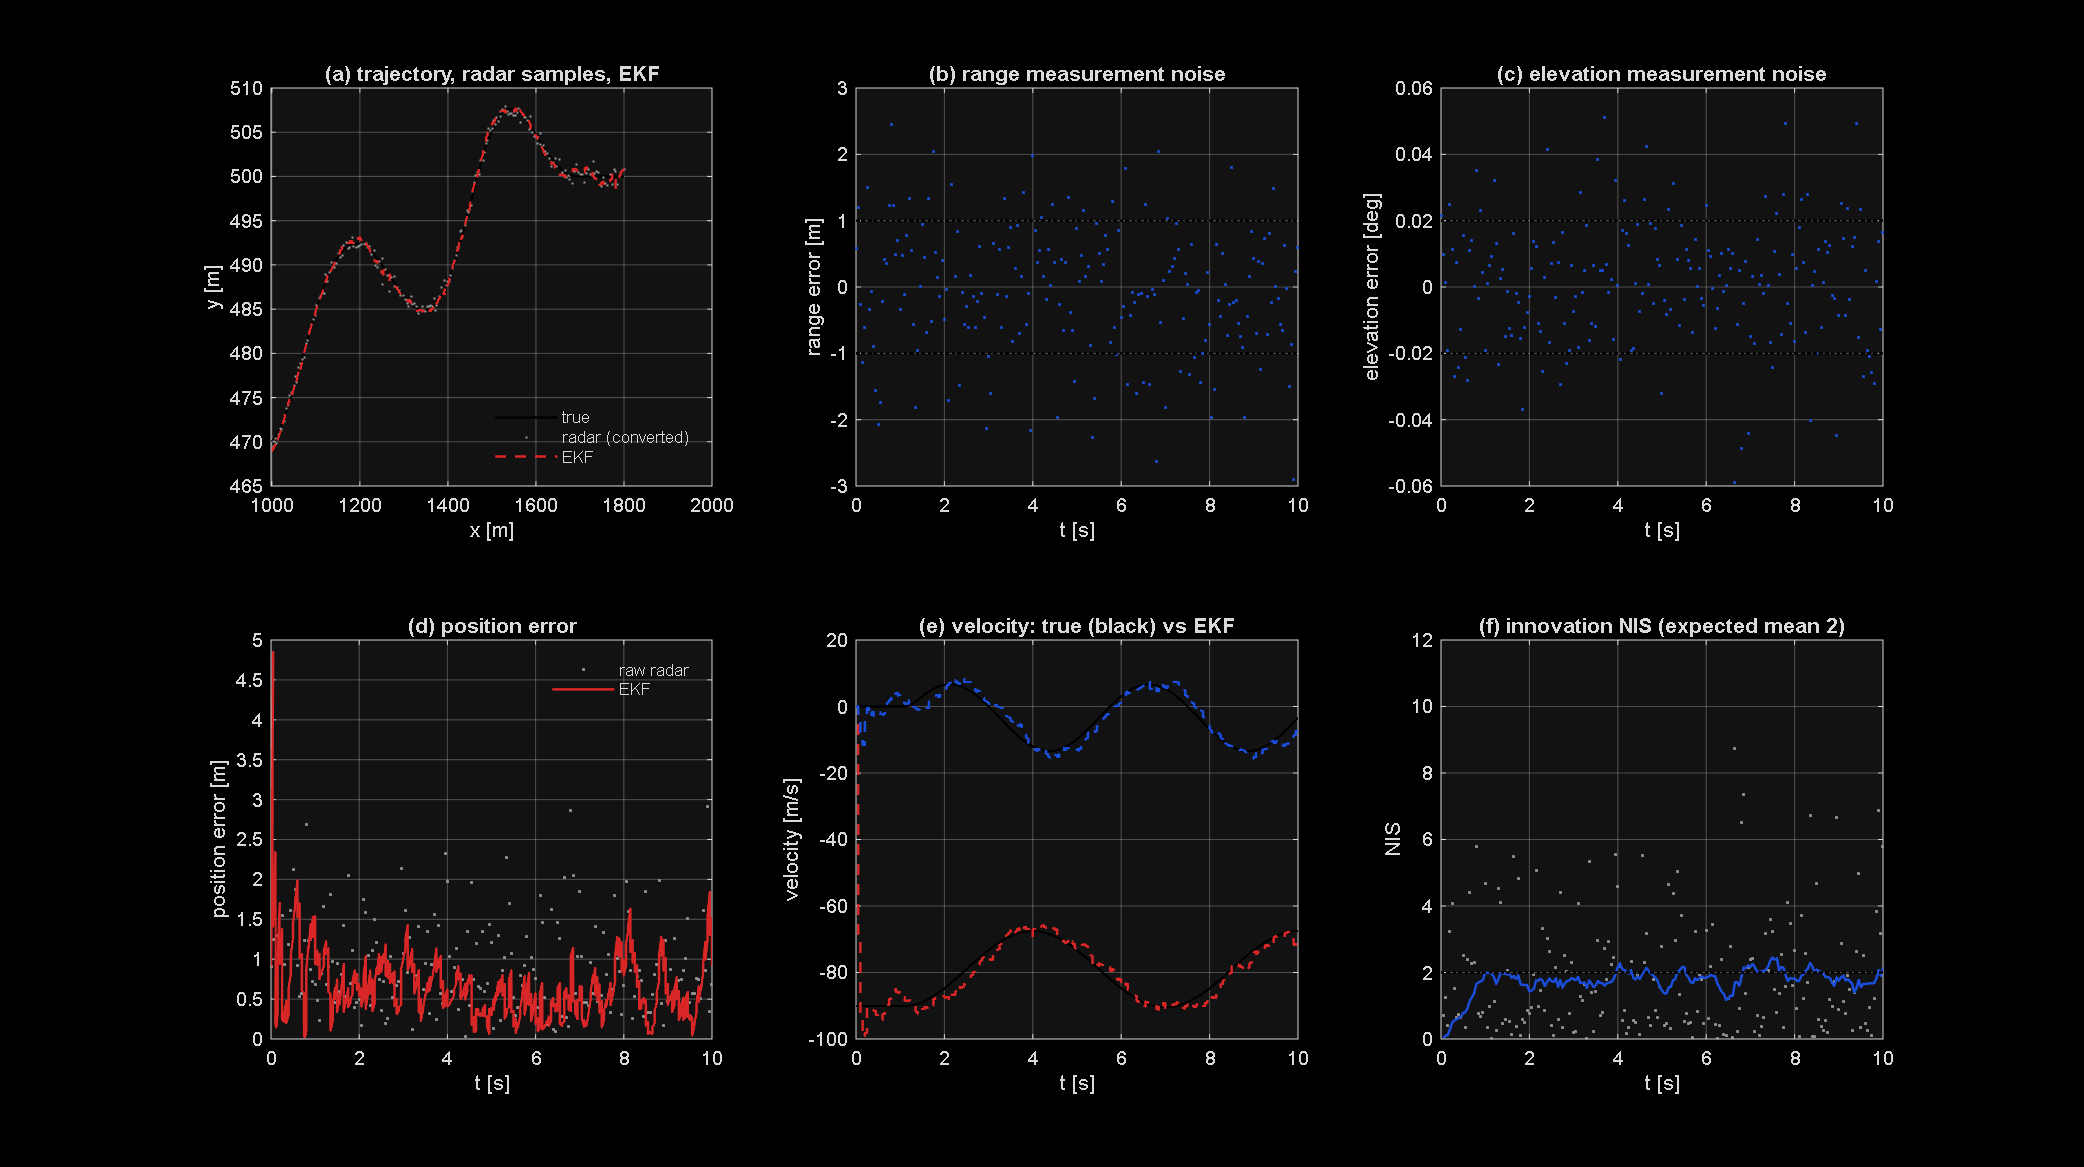
\includegraphics[width=0.56\textwidth]{fig_estimation.png}
\caption{Scenario B: (a) trajectory, radar samples, EKF; (b,c) range and elevation noise with $\pm1\sigma$ (dotted); (d) position error, raw vs.\ EKF; (e) velocity components; (f) innovation NIS.}\label{fig:est}
\end{figure*}
\begin{figure*}[t]
\centering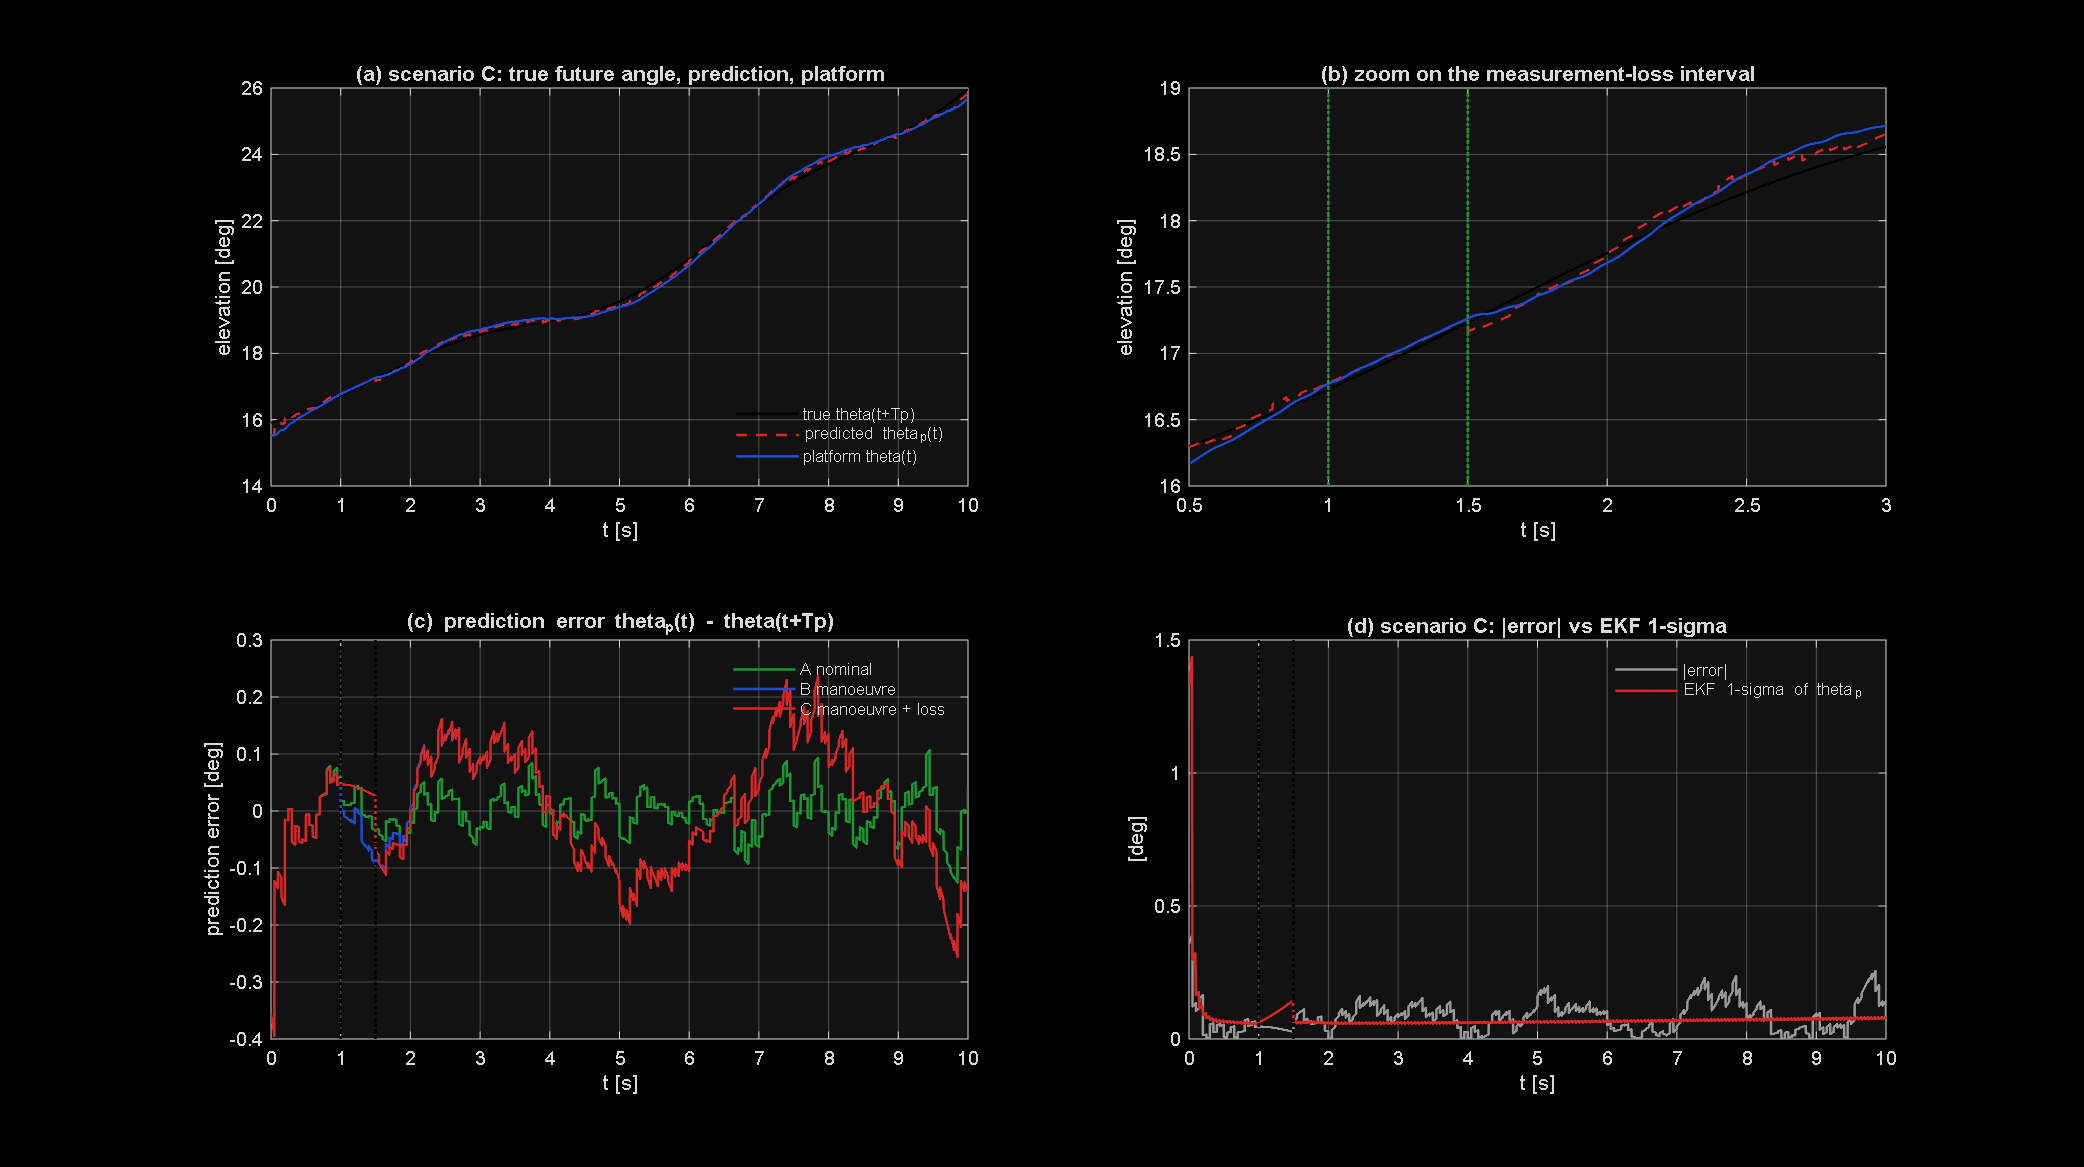
\includegraphics[width=0.56\textwidth]{fig_prediction.png}
\caption{Prediction: (a,b) scenario C true future angle, prediction and platform angle, with a zoom on the loss interval (dotted lines); (c) prediction error for A, B, C; (d) |error| against the EKF $1\sigma$.}\label{fig:pred}
\end{figure*}
\begin{figure*}[t]
\centering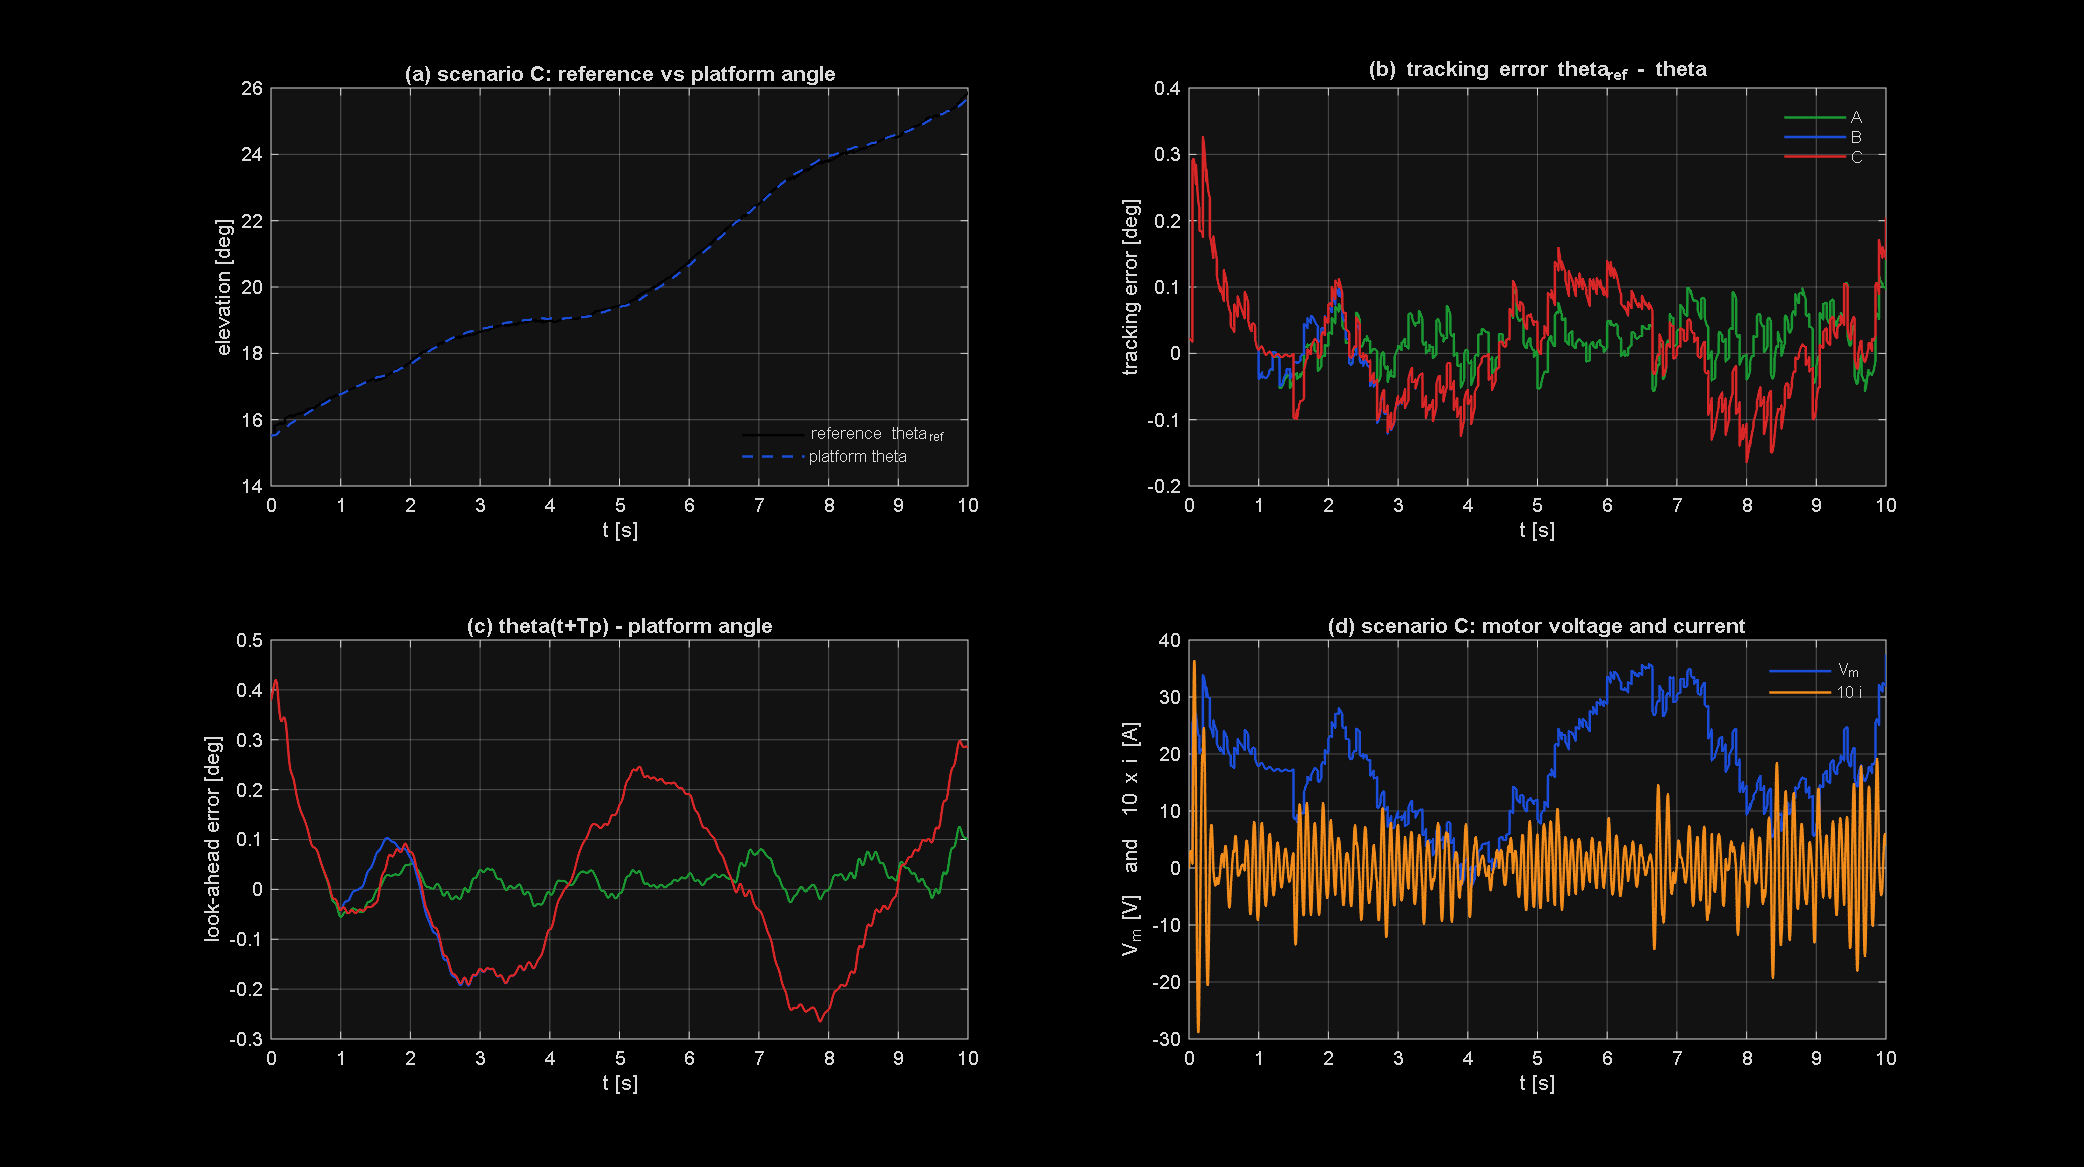
\includegraphics[width=0.56\textwidth]{fig_turret.png}
\caption{Platform response: (a) reference and platform angle (C); (b) tracking error; (c) look-ahead error; (d) motor voltage and current (C).}\label{fig:turret}
\end{figure*}
\begin{figure}[t]
\centering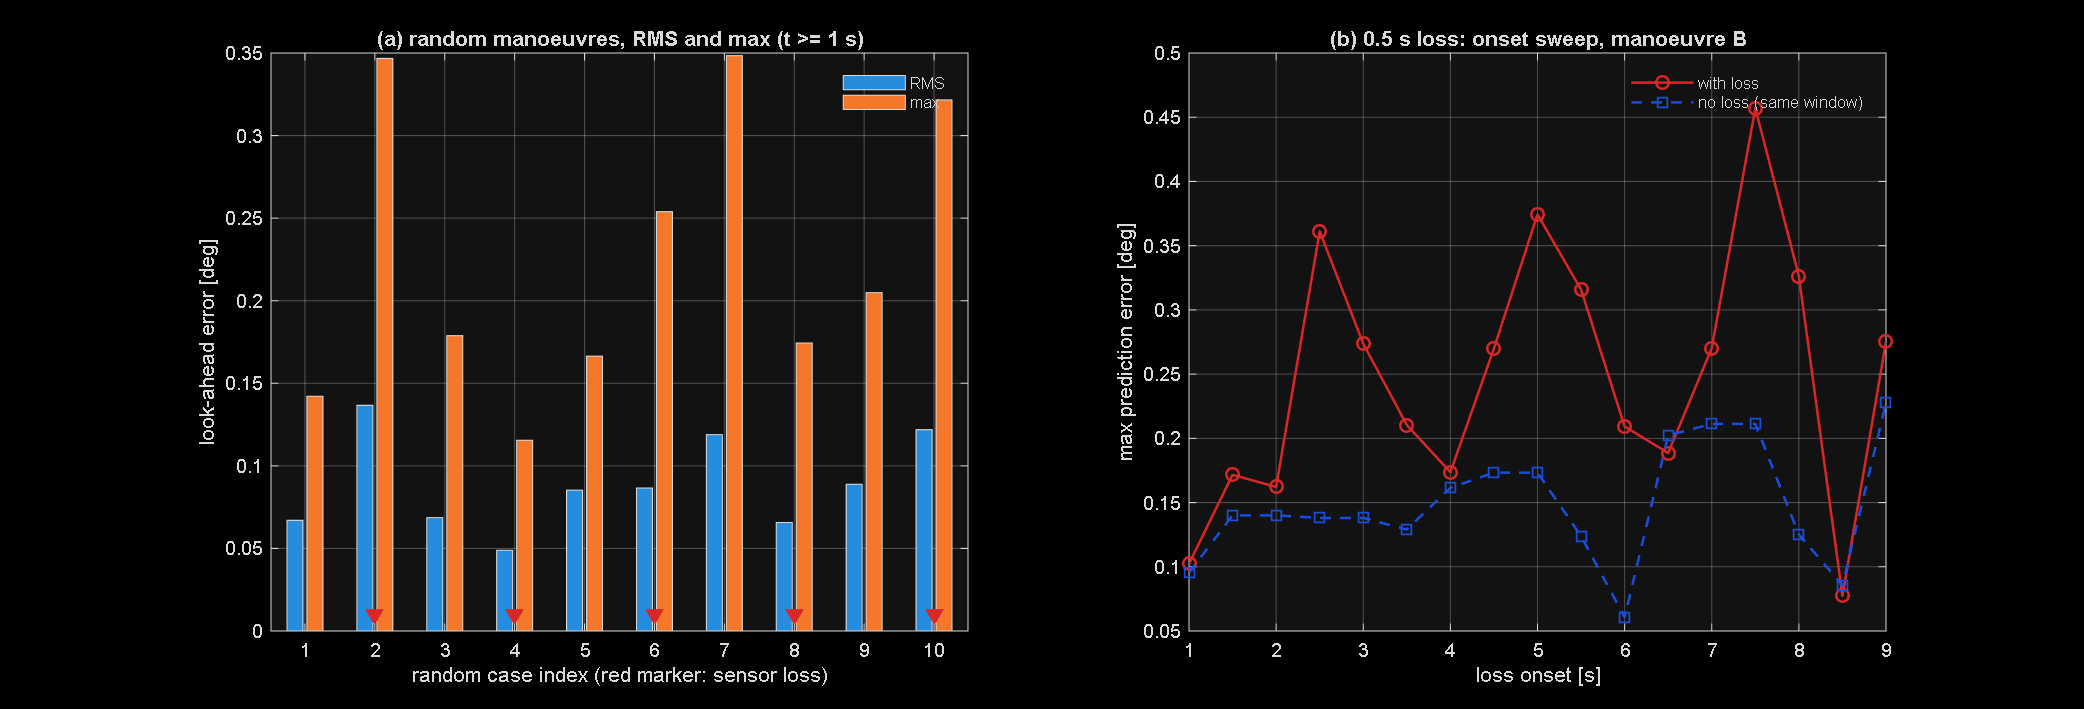
\includegraphics[width=\columnwidth]{fig_robustness.png}
\caption{Generalisation: (a) random manoeuvres; (b) loss-onset sweep.}\label{fig:rob}
\end{figure}

\section{Conclusions}
An EKF on a Singer model, open-loop extrapolation to $t+T_p$ and a PI compensator give a look-ahead error of about $0.15\dg$ RMS on a manoeuvring target, survive a 0.5 s radar loss, and intercepted 10 of 10 unseen cases under our scoring assumption. The main strengths are that each design number can be traced to a calculation (the bandwidth limit from the resonance, and the Routh gain limit agreeing with the numerical gain margin), and that the design worked on unseen manoeuvres without retuning. The main limitations are: the plant is idealised (no gravity, compliance, backlash or encoder noise); the voltage limit is our assumption; the test manoeuvres are smooth and not adversarial; the EKF assumes Gaussian noise; the loss timing in scenario C is mild; the firing gate was tuned on only 16 cases; the scoring convention for a pulse is an assumption; and everything is simulation only. Performance is limited mostly by the mismatch between the motion model and the real manoeuvre during a loss, and by the servo bandwidth that the resonance allows.

\bibliographystyle{IEEEtran}
\bibliography{references}

\clearpage
\appendix[Use of AI and Computational Tools]
\small
\textbf{Tools.} Anthropic Claude (Sonnet 5.5, claude.ai) was used as a coding and writing assistant. GNU Octave 8.4 was used for simulation and plotting, and TeX Live for typesetting.

\textbf{Done by the team.} We derived the mathematical model and design by hand (handwritten derivations available): the geared DC-motor plant $G_p(s)$ from the electrical and mechanical equations, the equivalent inertia, the target motion and Singer-model equations, the EKF formulation, the extrapolation to $t+T_p$, and the PI compensator design. We chose the design approach and told the AI what to implement and how, ran and tested all simulations ourselves, and directed the changes made after review: adding firing logic and interception metrics, removing the code that wrote LaTeX, and copying the paper's numbers by hand from the CSV files in \texttt{results/data}.

\textbf{Done by the AI.} Following our instructions, Claude wrote the Octave code (plant, estimator, predictor, controller, firing gate, automated checks, figures), ran the estimator-parameter and firing-gate tuning scripts and reported their results to us, set up the LaTeX, and drafted and rewrote the report wording from our results.

\textbf{Checks.} Our hand calculations were compared with the simulated results. The code also runs ten automated checks before each simulation (units, transfer function against state space, closed-form $\omega_n,\zeta$, energy balance, EKF Jacobian against finite differences, noise-free prediction, Routh limit against the numerical gain margin). The EKF innovation statistic (NIS) was close to 2, and the firing gate was replayed offline against the in-loop gate.

\textbf{Limits.} Results are Octave simulations only. The tuning set, scenarios and random test cases are separate. The pulse-scoring convention (target at $t_{fire}+T_p$) is an assumption not confirmed with the instructor.

\end{document}
